  \documentclass{beamer}
  \usepackage[utf8]{inputenc}
  \usepackage[frenchb]{babel}
  \usepackage{amsmath,amssymb}
  \usetheme{Warsaw}
% costumiser les bas de pages en ajoutant les nombre de pages...
  \setbeamertemplate{footline}{
  \leavevmode%
  \hbox{\hspace*{-0.06cm}
  \begin{beamercolorbox}[wd=.2\paperwidth,ht=2.25ex,dp=1ex,center]{author in head/foot}%
	  \usebeamerfont{author in head/foot}\insertshortauthor%~~(\insertshortinstitute)
  \end{beamercolorbox}%
  \begin{beamercolorbox}[wd=.5\paperwidth,ht=2.25ex,dp=1ex,center]{section in head/foot}%
	  \usebeamerfont{section in head/foot}\insertshorttitle
  \end{beamercolorbox}%
  \begin{beamercolorbox}[wd=.3\paperwidth,ht=2.25ex,dp=1ex,right]{section in head/foot}%
	  \usebeamerfont{section in head/foot}\insertshortdate{}\hspace*{2em}
	  \insertframenumber{} / \inserttotalframenumber\hspace*{2ex}
  \end{beamercolorbox}}%
  \vskip0pt%
  }

  \newtheorem{de}{Définition}
  \newtheorem{proposition}{Proposition}
  \newtheorem{theo}{Théorème}
  \title{Tables 0/1 Associées Aux Treillis Démontables}
  \author{Ismaeil Abouljamal}
  \date{08 Septembre 2011}
  \logo{test}
  \institute{LIF (UMR 6166)}
  %logos

\pgfdeclareimage[height=0.6cm]{left-logo}{images/ecm}
\pgfdeclareimage[height=0.6cm]{right-logo}{images/lif.jpeg}
\logo{\pgfuseimage{right-logo}}

\setbeamertemplate{sidebar left}
{
\logo{\pgfuseimage{left-logo}}
\vfill%
\rlap{\hskip0.1cm\insertlogo}%
\vskip15pt%
}
  \begin{document}
  \begin{frame}
  \titlepage
  \begin{center}
  {Encadrant : François Brucker}
  \end{center}
  \end{frame}
 
  \begin{frame}{Plan}
  \begin{enumerate}
   \item Introduction	
   \item Contexte Général
   \item Contribution
   \item Conclusions et Perspectives
   \end{enumerate}
  \end{frame}

%%%%%%%%%%%%%%%%%%%%%%%%%%%%%
%%% Introduction
%%%%%%%%%%%%%%%%%%%%%%%%%%%%%
  \begin{frame}{Introduction}
  \og Le seul moyen de faire une méthode instructive et naturelle est de \textbf{mettre ensemble} les choses qui se ressemblent et de \textbf{séparer} celles qui diffèrent
  les unes des autres\fg 

  (Georges Louis Leclerc de Buffon. \textsc{Histoire Naturelle}).
  \end{frame}

  \begin{frame}{Introduction}
  \LARGE {\textrm{Hiérarchies}}

  $A \cap B \in \{A, B, \varnothing\}$
   \begin{figure}
	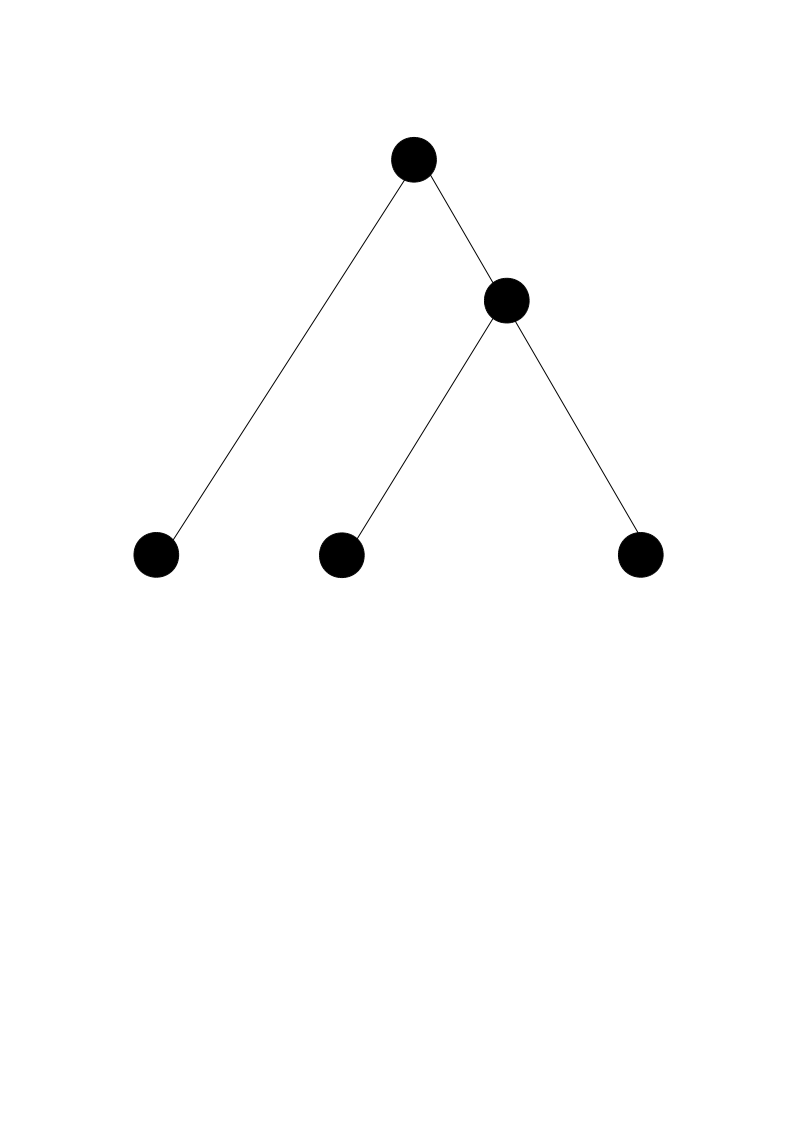
\includegraphics[width=7cm]{images/memoire_figure0_treillis.png} 
    \end{figure}
  \end{frame}

  \begin{frame}{Introduction}
  \LARGE {\textrm{Empiétances}}
   \begin{figure}
	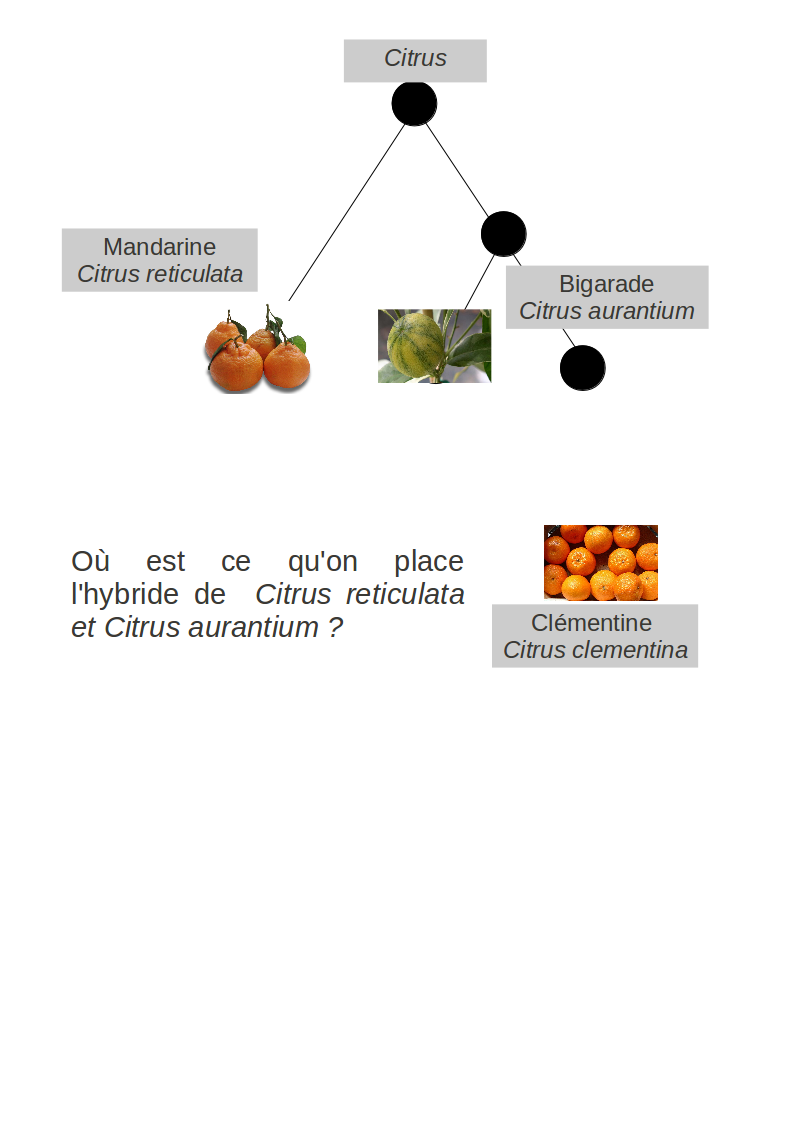
\includegraphics[width=7cm]{images/memoire_figure5.png} 
    \end{figure}
  \end{frame}


  \begin{frame}{Introduction}
  \LARGE {\textrm{Hiérarchie Faible}}

  $A \cap B \cap C\in \{A \cap B, B \cap C, A \cap C\}$
   \begin{figure}
	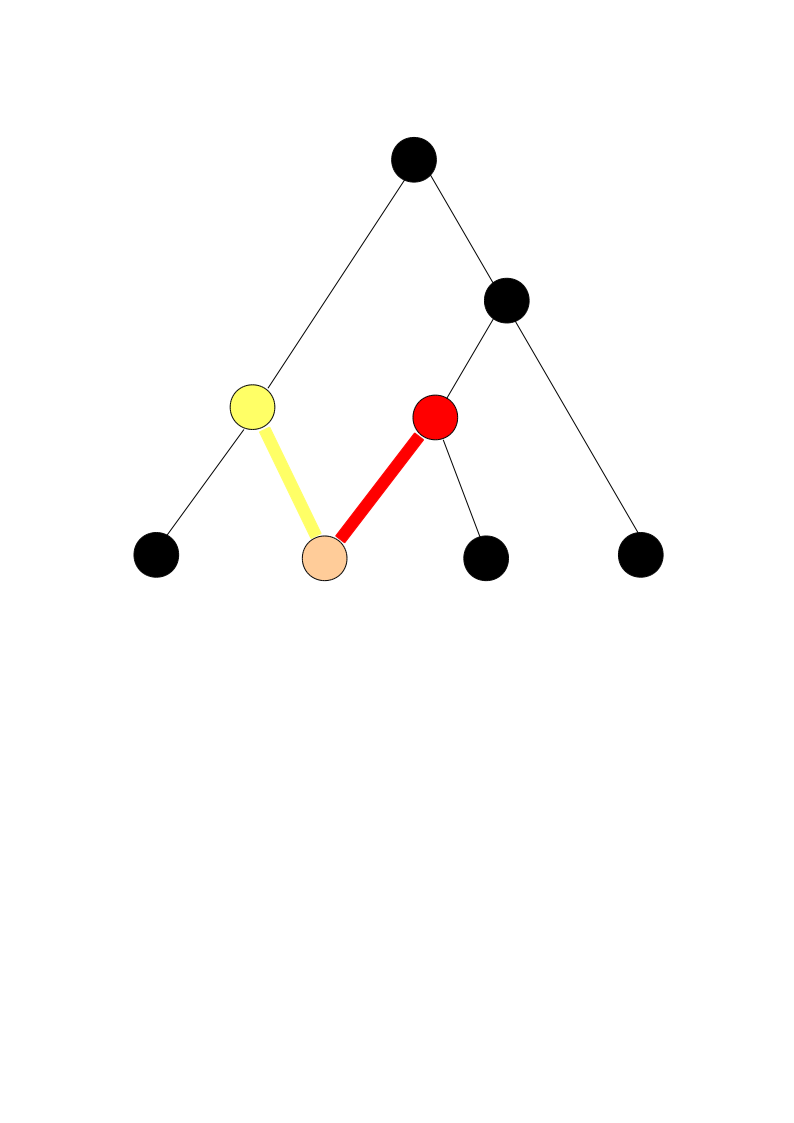
\includegraphics[width=7cm]{images/memoire_figure2.png} 
    \end{figure}
  \end{frame}

  \begin{frame}{Introduction}
  \LARGE {\textrm{Hybridation}}
   \begin{figure}
	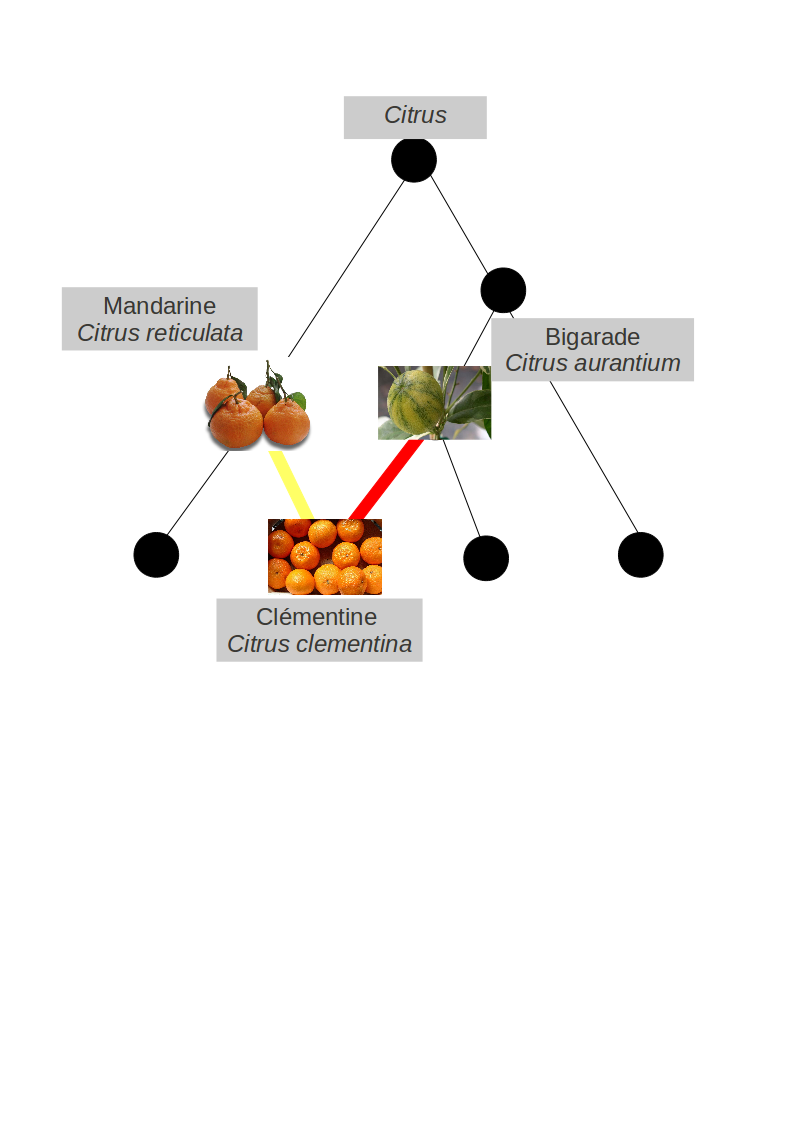
\includegraphics[width=8cm]{images/memoire_figure3.png} 
    \end{figure}
  \end{frame}

  \begin{frame}{Introduction}
  \LARGE {\textrm{Treillis}}
   \begin{figure}
   	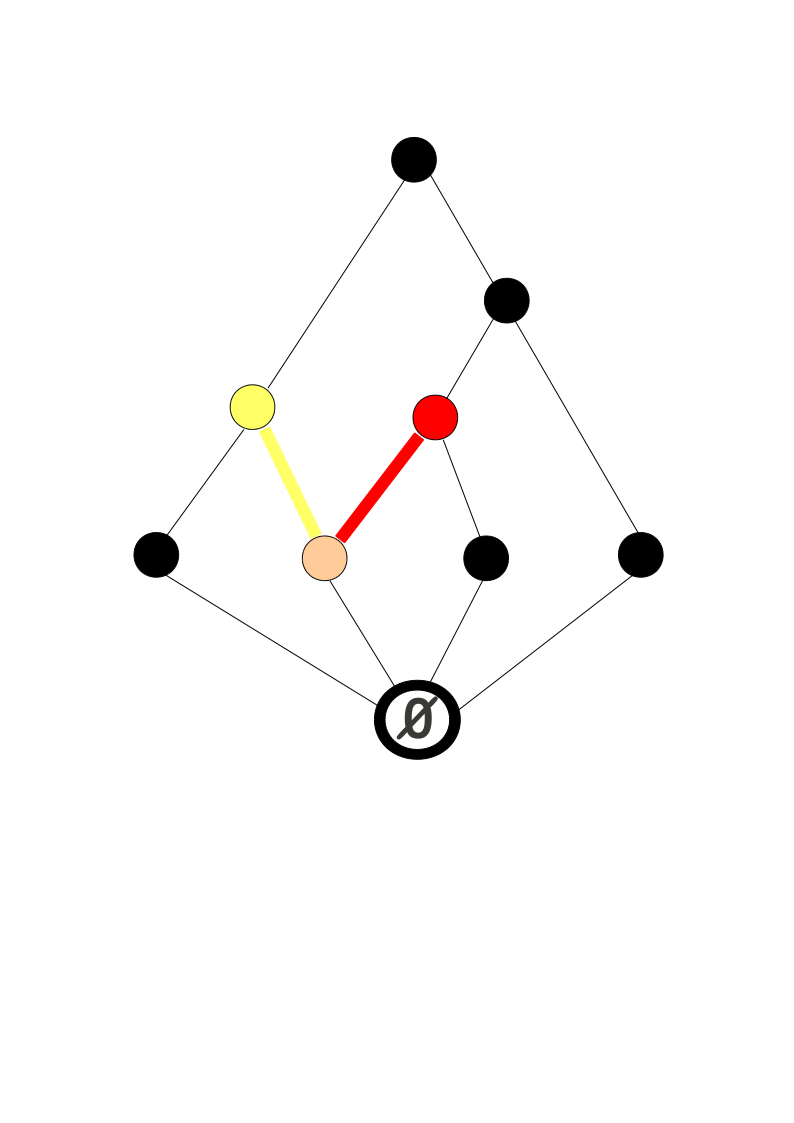
\includegraphics[width=7cm]{images/memoire_figure2_treillis.png}
   \end{figure}
  \end{frame}


  \begin{frame}{Introduction}
  \LARGE {\textrm{Treillis Démontables}}
   \begin{figure}
	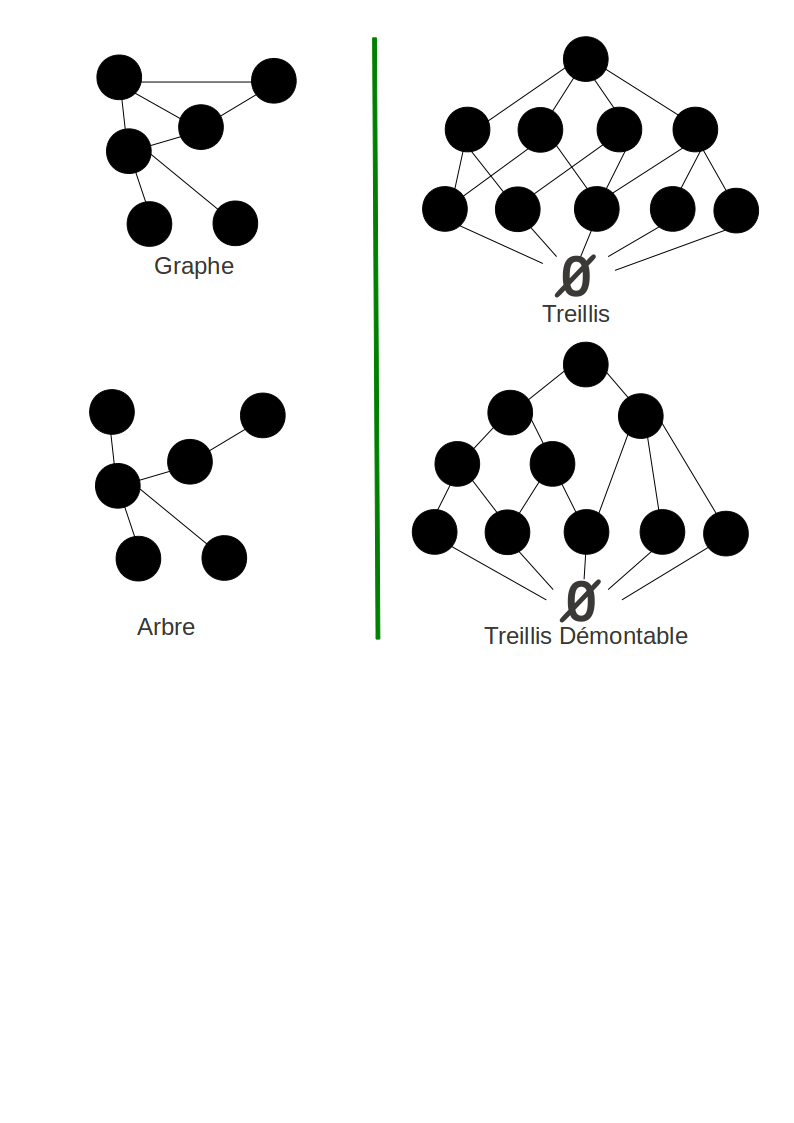
\includegraphics[width=8cm]{images/memoire_figure4.png} 
    \end{figure}
  \end{frame}

  \begin{frame}{Introduction}
  \LARGE {\textrm{Motivation}}
   \begin{figure}
	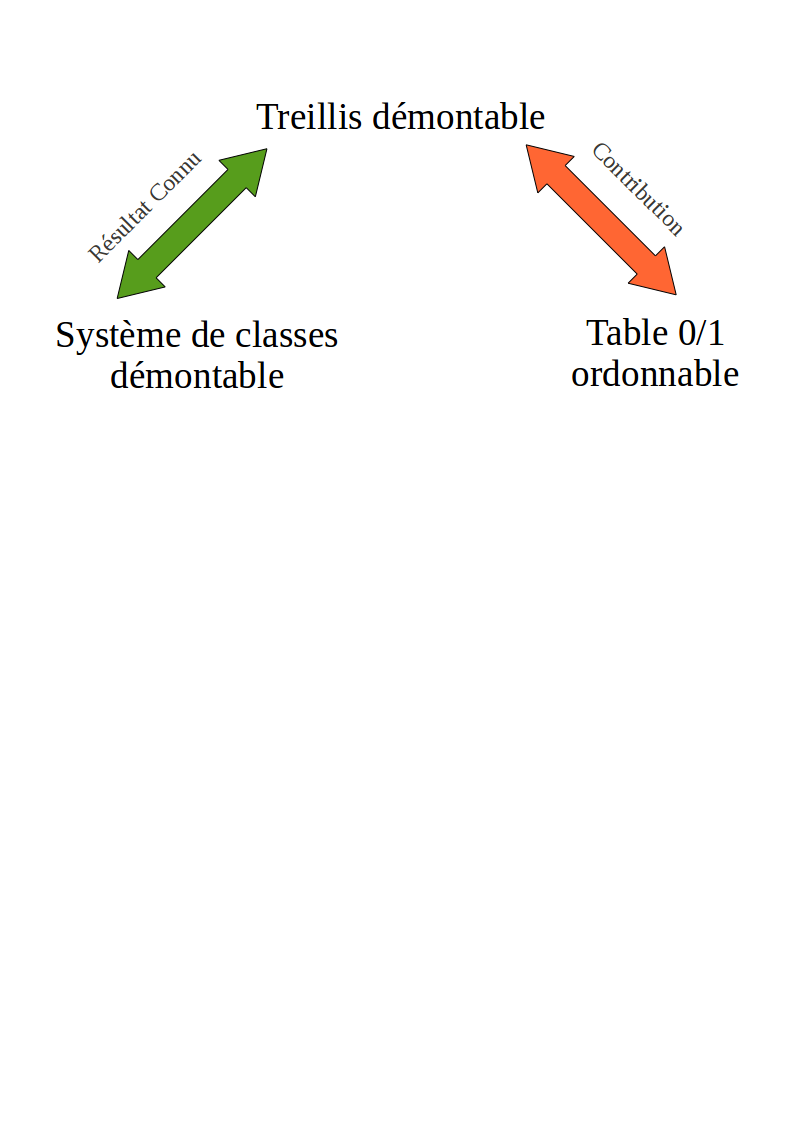
\includegraphics[width=8cm]{images/memoire_figure6.png} 
    \end{figure}
  \end{frame}
%%%%%%%%%%%%%%%%%%%%%%%%%%%%%
%%% Contexte Général
%%%%%%%%%%%%%%%%%%%%%%%%%%%%%
  \begin{frame}{Contexte Général}
  \framesubtitle{Treillis démontable}
   \begin{figure}
	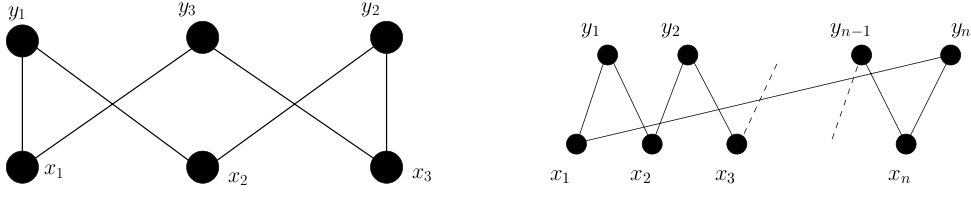
\includegraphics[width=8cm]{images/3c.png} 
    \end{figure}

	\begin{theo}[Treillis démontable(Kelly et Rival 1974)]
	Un treillis est démontable s'il n'a pas de couronne.
	\end{theo}
  \end{frame}

  \begin{frame}{Contexte Général}
  \framesubtitle{Treillis démontable}
	\begin{de}[Treillis démontable (Rival 1974)]
	Un treillis $T = (E, \leq)$ est démontable s'il existe un élément doublement irréductible $x \in E$ tel que 
	le treillis $T = (E \backslash \{x\}, \leq)$ reste démontable.
	\end{de}
  \end{frame}

  \begin{frame}{Contexte Général}
  \framesubtitle{Treillis démontable}
   \begin{figure}
	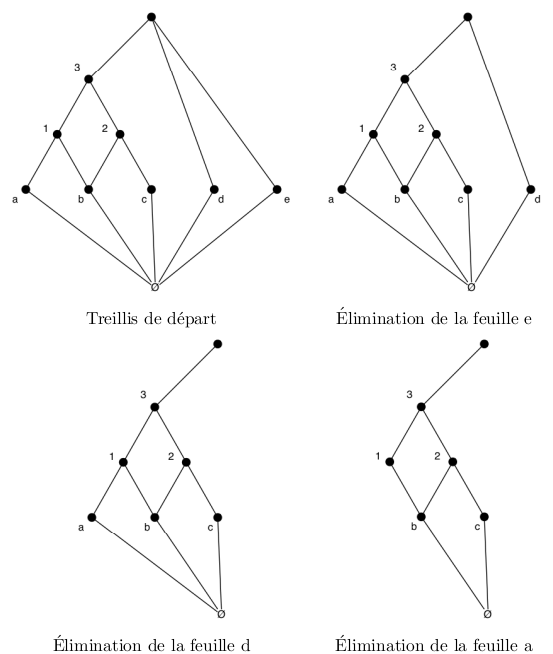
\includegraphics[width=6cm]{images/e_tr_1.png} 
    \end{figure}
  \end{frame}

  \begin{frame}{Contexte Général}
  \framesubtitle{Treillis démontable}
   \begin{figure}
	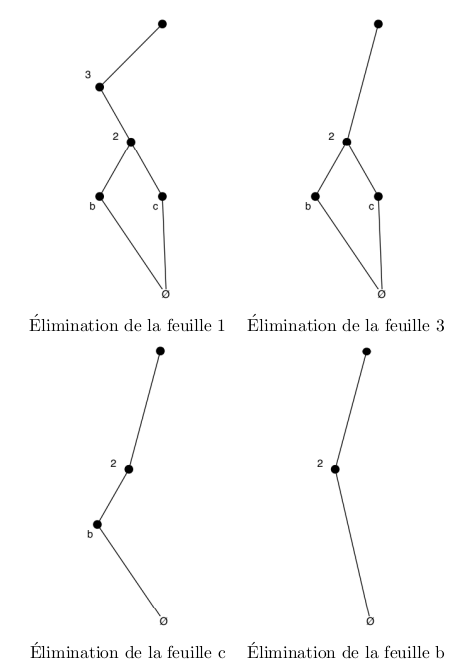
\includegraphics[width=5cm]{images/e_tr_2.png} 
    \end{figure}
  \end{frame}

  \begin{frame}{Contexte Général}
  \framesubtitle{Système de classes démontable}
  \begin{de}[Feuille sur un système de classes]
  un élément $i \in X$ est une feuille sur un système de classes $F$ si son filtre  $\uparrow i$ forme une cha\^ine.
  \end{de}
   \begin{figure}
	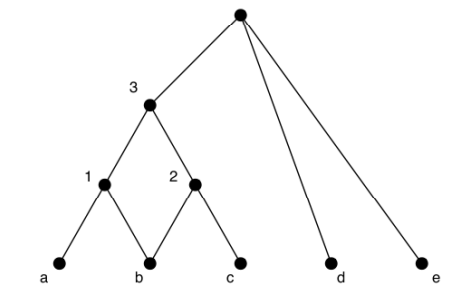
\includegraphics[width=5cm]{images/fl.png} 
    \end{figure}
  \end{frame}


  \begin{frame}{Contexte Général}
  \framesubtitle{Système de classes démontable}
  \begin{de}[Système de classes démontable]
  Un système de classe $\mathcal{H}$ est démontable s'il contient une feuille $x$ tel que $\mathcal{H} \backslash \{x\}$ 
  reste démontable.
  \end{de}
  \end{frame}

  \begin{frame}{Contexte Général}
  \framesubtitle{Système de classes démontable}
   \begin{figure}
	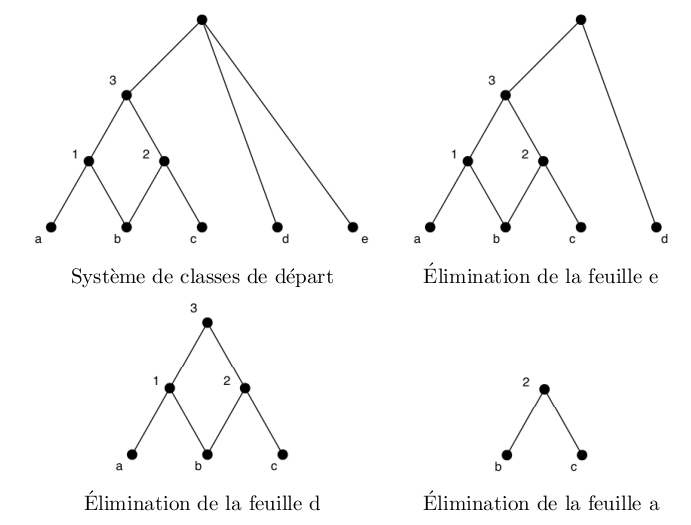
\includegraphics[width=8cm]{images/e_sc.png} 
    \end{figure}
  \end{frame}

  \begin{frame}{Contexte Général}
  \framesubtitle{Treillis démontable $\Leftrightarrow$ Système de classes associé démontable}
\begin{itemize}
 \item   Soit un treillis démontable associé au système de classes $\mathcal{H}$.

  Si on enlève la feuille $x$ au treillis, le système de classes associé est $\mathcal{H} \backslash \{x\}$.
 \item Treillis démontable $\Leftrightarrow$ Système de classes associé démontable.
\end{itemize}


 
  \end{frame}
%%%%%%%%%%%%%%%%%%%%%%%%%%%%%
%%% Contribution
%%%%%%%%%%%%%%%%%%%%%%%%%%%%%
  \begin{frame}{Contribution}
  \framesubtitle{Correspondance de Galois}
\begin{table}[htb]
  \centering

\begin{tabular}{lccccc}
 & $a_1$ & $a_2$ & $a_3$ & $a_4$ & $a_5$\\
$x_1$ & \textbf{1} & \textbf{1} & \textbf{0} & \textbf{0} & \textbf{0}\\
$x_2$ & \textbf{1} & \textbf{0} & \textbf{1} & \textbf{0} & \textbf{0}\\
$x_3$ & \textbf{0} & \textbf{1} & \textbf{1} & \textbf{1} & \textbf{0}\\
$x_4$ & \textbf{0} & \textbf{0} & \textbf{0} & \textbf{1} & \textbf{1}\\
$x_5$ & \textbf{0} & \textbf{0} & \textbf{0} & \textbf{1} & \textbf{0}

\end{tabular}
\caption{Exemple de table 0/1  }
\end{table}
  \end{frame}

  \begin{frame}{Contribution}
  \framesubtitle{Correspondance de Galois}
   \begin{figure}
	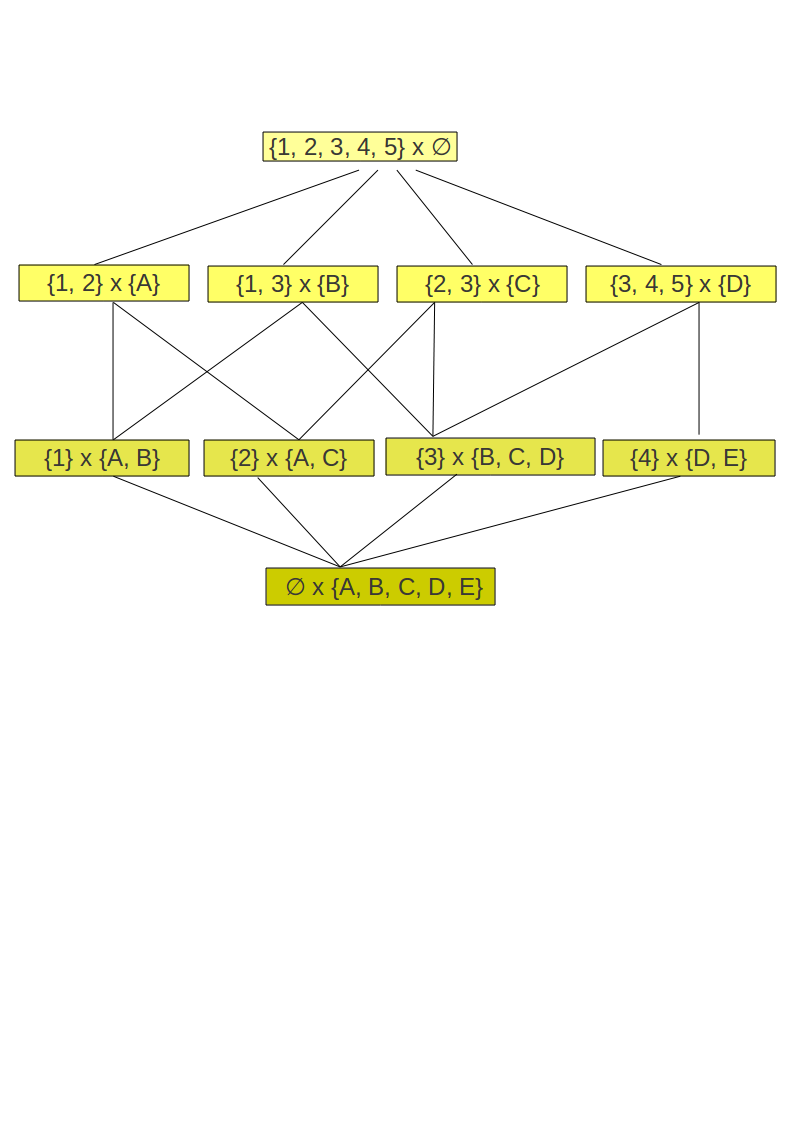
\includegraphics[width=8cm]{images/treillis.png} 
    \end{figure}
  \end{frame}

  \begin{frame}{Contribution}
  \framesubtitle{Correspondance de Galois}
   \begin{figure}
	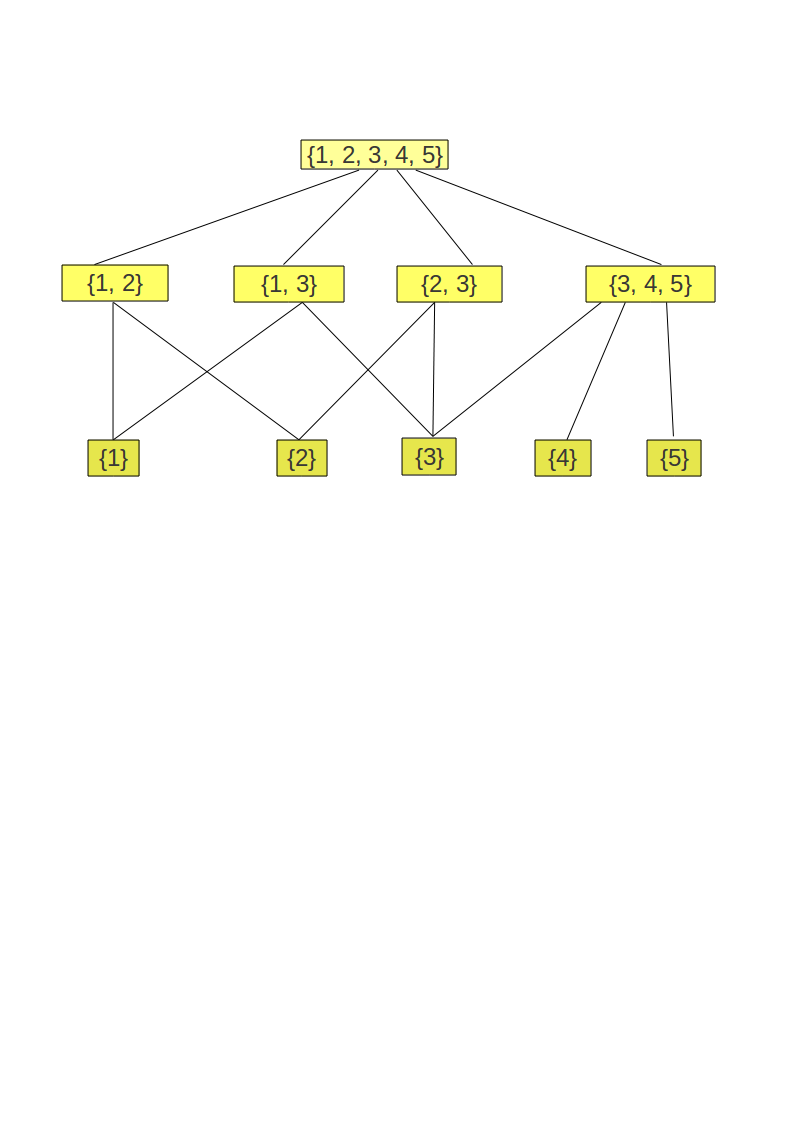
\includegraphics[width=8cm]{images/treillismoins.png} 
    \end{figure}
  \end{frame}

  \begin{frame}{Contribution}
  \framesubtitle{Configuration $\Gamma$}
  \begin{de}[Configuration $\Gamma$]
  Pour tout $(i, j, j')$ tel que $1 \leq i \leq n$ et $1 \leq j < j' \leq m$,\\
  Si $T_{(i, j')} = T_{(i, j)} = 1$ Alors $\forall i'\geqslant i, T_{(i', j)} = 1 \Rightarrow T_{(i', j')} = 1$.
  \end{de}

  \begin{table}[htb]
  \centering
  \begin{tabular}{*{4}{c|} c}
  
	$\cdots$ & $j$ & $\cdots$ & $j'$ & $\cdots$\\
  \hline
	$i$ & 1 & $\cdots$ & 1 & $\cdots$\\
  \hline
	$\cdots$ & * & $\cdots$ & * & $\cdots$\\
  \hline
	$i'$ & 1 & $\cdots$ & 0 & $\cdots$
  \end{tabular}
  \caption{Configuration $\Gamma$}
  \label{gammma}
  \end{table}
  \end{frame}

  \begin{frame}{Contribution}
  \framesubtitle{Table ordonnable}
  \begin{de}[Table bien ordonnée]
  Une Table 0/1 qui ne contient pas de configuration $\Gamma$ est appelée
  table \textit{bien ordonnée}.
  \end{de}

  \begin{de}[Table ordonnable]
  Une Table 0/1 $T$ est \textit{ordonnable} si et seulement s'il existe une permutation $\sigma_L$ sur les lignes 
  et une permutation $\sigma_C$ sur les colonnes telles que~:
  la table $T'$ définie par $T'_{(i, j)} = T_{(\sigma_L(i), \sigma_C(j))}$ pour tout $(i, j)$ entiers naturels 
  non nuls soit bien ordonnée.
  \end{de}
  \end{frame}

  \begin{frame}{Contribution}
  \framesubtitle{Exemple Table ordonnable}
	\begin{table}[htb]
	  \centering

	\begin{tabular}{lccccc}
	& $a''_1$ & $a''_2$ & $a''_3$ & $a''_4$ & $a''_5$\\
	$x''_1$ & \textbf{1} & \textbf{1} & \textbf{0} & \textbf{0} & \textbf{0}\\
	$x''_2$ & \textbf{1} & \textbf{1} & \textbf{1} & \textbf{0} & \textbf{0}\\
	$x''_3$ & \textbf{0} & \textbf{1} & \textbf{1} & \textbf{1} & \textbf{0}\\
	$x''_4$ & \textbf{0} & \textbf{0} & \textbf{0} & \textcolor{red}{\textbf{1}} & \textcolor{red}{\textbf{1}}\\
	$x''_5$ & \textbf{0} & \textbf{0} & \textbf{0} & \textcolor{red}{\textbf{1}} & \textbf{0}
	\end{tabular}
  \caption{Configuration $\Gamma$ sur $x''_4$ et $x''_5$ }
	\end{table}
  \end{frame}

  \begin{frame}{Contribution}
  \framesubtitle{Exemple Table bien ordonnée}
	\begin{table}[htb]
	  \centering

	\begin{tabular}{lccccc}
	& $a'''_1$ & $a'''_2$ & $a'''_3$ & $a'''_4$ & $a'''_5$\\
	$x'''_1$ & \textbf{1} & \textbf{1} & \textbf{0} & \textbf{0} & \textbf{0}\\
	$x'''_2$ & \textbf{1} & \textbf{1} & \textbf{1} & \textbf{0} & \textbf{0}\\
	$x'''_3$ & \textbf{0} & \textbf{1} & \textbf{1} & \textbf{1} & \textbf{0}\\
	$x'''_4$ & \textbf{0} & \textbf{0} & \textbf{0} & \textbf{1} & \textbf{0}\\
	$x'''_5$ & \textbf{0} & \textbf{0} & \textbf{0} & \textbf{1} & \textbf{1}
	\end{tabular}
   \caption{Absence de configuration $\Gamma$}
	\end{table}
  \end{frame}

  \begin{frame}{Contribution}
  \framesubtitle{Feuille sur une table}
  \begin{de}[Feuille sur une table 0/1]
  Un individu $x_i$ est une feuille sur une table 0/1 $T$ si ses classes s'emboitent~:
  $\forall (a_j, a_j') \in Attr(x_i)^2, Ind(a_j) \subseteq Ind(a_j')$ ou $Ind(a_j') \subseteq Ind(a_j)$.
  \footnote{$Attr(x_i) =$ ensemble des attributs de $x_i$, et $Ind(a_j) =$ ensemble des individus qui ont l'attribut $a_j$}
  \end{de}
  \begin{table}[htb]
	\centering
  \begin{tabular}{lccccc}
  & $a_1$ & $a_2$ & $a_3$ & $a_4$ & $a_5$\\
  $x_1$ & \textbf{1} & \textbf{1} & \textbf{0} & \textbf{0} & \textbf{0}\\
  $x_2$ & \textbf{1} & \textbf{0} & \textbf{1} & \textbf{0} & \textbf{0}\\
  $x_3$ & \textbf{0} & \textbf{1} & \textbf{1} & \textbf{1} & \textbf{0}\\
  $x_4$ & \textbf{0} & \textbf{0} & \textbf{0} & \textbf{1} & \textbf{1}\\
  $x_5$ & \textbf{0} & \textbf{0} & \textbf{0} & \textbf{1} & \textbf{0}
  \end{tabular}
  \caption{$x_4$ est une feuille car $Ind(a_5)$ est inclus dans $Ind(a_4)$.}
  \end{table}

  \end{frame}

  \begin{frame}{Contribution}
  \framesubtitle{Configuration $\Gamma$}
  \begin{proposition}
  Une table 0/1 $T$ est bien ordonnée
  si et seulement si, 
  pour tout $(i, x_{i_0}, a_j, a_{j'})$ tels que: $1 \leq a_j < a_{j'} \leq m$ et $1 \leq x_{i_0} \leq i \leq n$
  \begin{equation}
  x_{i_0} \in Ind_{}(a_j) \cap Ind_{}(a_{j'}) 
  \Rightarrow
  Ind_{\geqslant x_{i_0}}(a_j) \subseteq Ind_{\geqslant x_{i_0}}(a_{j'})
  \label{hyp} 
  \end{equation}
  \end{proposition}

  \begin{table}
  \centering
  \begin{tabular}{*{7}{c|} c}
	%\backslashbox{Individu}{Classe}
	  & $\cdots$ & $a_j$ & $\cdots$ & $a_{j'}$  & $\cdots$ & $a_{j'}'$ & $\cdots$\\
  \hline
	$i$ & $\cdots$ & $///$ & $\cdots$ & $///$  & $\cdots$ & $///$  & $\cdots$\\
  \hline
	$\vdots$ & $\vdots$ & $\vdots$ & $\vdots$ & $\vdots$  & $\vdots$ & $\vdots$ & $\vdots$\\
  \hline
	$x_{i_0}$ & $\cdots$ & 1 & $\cdots$ & 1 & $\cdots$ & 1 & $\cdots$\\
  \hline
	$x_{i_0} + 1$ & $\cdots$ & 0 & $\cdots$ & 1 & $\cdots$ & 1 & $\cdots$\\
  \hline
	$x_{i_0} + 2$ & $\cdots$ & 0 & $\cdots$ & 0 & $\cdots$ & 1 & $\cdots$\\
  \hline
	$x_{i_0} + 3$ & $\cdots$ & 1 & $\cdots$ & 1 & $\cdots$ & 1 & $\cdots$\\
  \end{tabular}
  \caption{Illustration de l'équation~\ref{hyp}}
  \end{table}
  \end{frame}

  \begin{frame}{Contribution}
  \framesubtitle{Correspondance des feuilles}
  \begin{proposition}[Correspondance des feuilles]
  \label{propfeuille}
  Soit $F$ le système de classes associé à une table 0/1 $T$.

  $x_i$ est une feuille sur $F$ 
  $\Leftrightarrow$
  $x_i$ est une feuille sur la table 0/1 $T$.
  \end{proposition}
  \end{frame}

  \begin{frame}{Contribution}
  \framesubtitle{Exemple correspondance des feuilles}
	\begin{table}[htb]
	  \centering

	\begin{tabular}{lccccc}
	& $a'''_1$ & $a'''_2$ & $a'''_3$ & $a'''_4$ & $a'''_5$\\
	$x'''_1$ & \textbf{1} & \textbf{1} & \textbf{0} & \textbf{0} & \textbf{0}\\
	$x'''_2$ & \textbf{1} & \textbf{1} & \textbf{1} & \textbf{0} & \textbf{0}\\
	$x'''_3$ & \textbf{0} & \textbf{1} & \textbf{1} & \textbf{1} & \textbf{0}\\
	$x'''_4$ & \textbf{0} & \textbf{0} & \textbf{0} & \textbf{1} & \textbf{0}\\
	$x'''_5$ & \textbf{0} & \textbf{0} & \textbf{0} & \textbf{1} & \textbf{1}
	\end{tabular}
   \caption{$x'''_1$ est une feuille car $Attr(x'''_1) =\{a'''_1, a'''_2\}$ et  $Ind(a'''_2)$ contient $Ind(a'''_1)$}
	\end{table}
  \end{frame}

  \begin{frame}{Contribution}
  \framesubtitle{Exemple correspondance des feuilles}
   $x'''_1$ est une feuille sur le treillis associé car son filtre forme une chaîne.
   \begin{figure}
	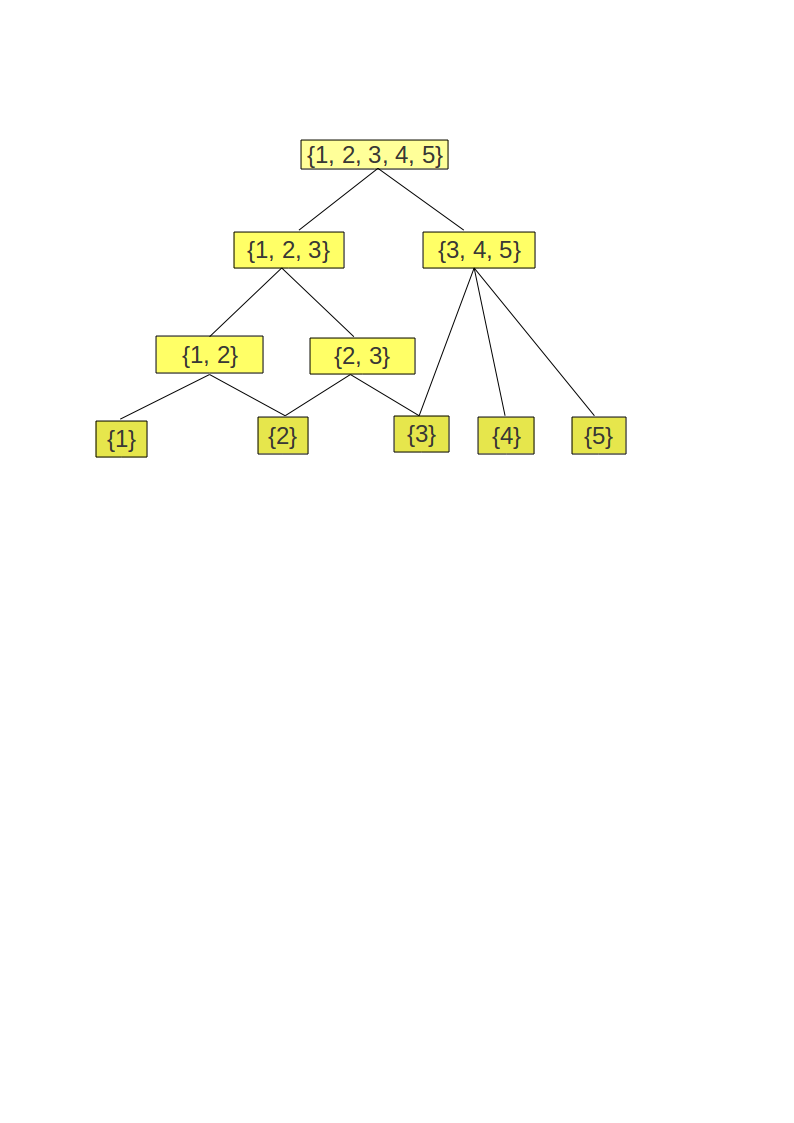
\includegraphics[width=8cm]{images/treillismoins2.png} 
    
    \end{figure}
   
  \end{frame}

  \begin{frame}{Contribution}
  \framesubtitle{Démontabilité $\Leftrightarrow$ Ordonnabilité}
  \begin{theo}[Ordonnabilité $\Leftrightarrow$ Démontabilité ]
  Soit $\mathcal{H}$ le système de classes associé à une table présence/absence $T$.

  $\mathcal{H}$ est démontable $\Leftrightarrow$ $T$ est ordonnable .  
  \end{theo}
  \end{frame}

  \begin{frame}{Contribution}
  \framesubtitle{Correspondance de restriction}
  \begin{theo}[Table restreinte]
  Soit $\mathcal{H} = (X, \mathcal{E})$ le système de classes associé à une table 0/1 $T$.
  Soit $T^{\star}$ la table $T$ privée de sa ligne $i$.
  Soit $\mathcal{H}^{\star}$ le système de classes associé à $T^{\star}$.
  On a alors~: 
  $\mathcal{H}^{\star} = \mathcal{H} \backslash \{x_i\}  =(X \backslash \{x_i\} , \mathcal{E}^{'})$.
  \end{theo}
  \end{frame}

  \begin{frame}{Contribution}
  \framesubtitle{Ordonnabilité $\Rightarrow$ Démontabilité}
  \begin{proposition}[Ordonnabilité - Démontabilité]
  Soit $\mathcal{H}$ le système de classes associé à une table présence/absence $T$.

  $T$ est ordonnable $\Rightarrow$ $\mathcal{H}$ est démontable. 
  \end{proposition}
  \end{frame}

  \begin{frame}{Contribution}
  \framesubtitle{Démontabilité $\Rightarrow$ Ordonnabilité}
  \begin{proposition}[Démontabilité - Ordonnabilité]
  Soit $\mathcal{H}$ le système de classes associé à une table présence/absence $T$.

  $\mathcal{H}$ est démontable $\Rightarrow$ $T$ est ordonnable. 
  \end{proposition}
  \end{frame}

  \begin{frame}{Contribution}
  \framesubtitle{Preuve}

\begin{enumerate}
\item $find\_order(\mathcal{H});$ trouver un ordre de démontage des individus de $\mathcal{H}$. (le premier à être démonté est $x_n$ et le dernier $x_1$).
\item $T' = lignes\_reorder(T);$ ordonner les lignes de la table $T$ dans l'ordre de démontabilité de $\mathcal{H}$ (la première ligne est $x_1$ et la dernière est $x_n$).
\item
\item 
\end{enumerate}

  \end{frame}

  \begin{frame}{Contribution}
  \framesubtitle{Preuve - Suite}

\begin{enumerate}
\item 
\item 
\item
  \begin{itemize}
	\item Soit la fonction  $colonnes\_reorder$ qui prend en entrée une table $Tab$ de $n$ lignes et $m$ colonnes, et une ligne $x_k$ comprise entre $x_1$ et $x_n$ ; et qui retourne
 une table $Result$.

		  $colonnes\_reorder(Tab, x_k)$
		  \begin{itemize}
		   \item $Result = Tab;$
		   \item $D =$ table dont des lignes sont ceux de $Result$ dans leur ordre et les colonnes sont les $Attr(x_k)$.
		   \item $G =$ table dont des lignes sont ceux de $Result$ dans leur ordre et les colonnes sont les attributs $a$ tel que $a \notin Attr(x_k)$.
		   \item Si $|G.colonnes| > 1$ et $k > 1$, alors $colonnes\_reorder(G, x_{k-1});$
		   \item Si $|D.colonnes| > 1$ et $k > 1$, alors $colonnes\_reorder(D, x_{k-1});$
           \item $Result = concatenate (G, D);$ 
		  \end{itemize}
		  $return$~$Result;$
  \end{itemize}
\item $TableOrdonnee = colonnes\_reorder(T', x_n);$
\end{enumerate}

  \end{frame}

  \begin{frame}{Contribution}
  \framesubtitle{Preuve - Illustration - étape 1 et 2}
\begin{table}[htb]
  \centering
\begin{tabular}{lccccc}
 & $a'''_1$ & $a'''_2$ & $a'''_3$ & $a'''_4$ & $a'''_5$\\
$x'''_1$ & \textbf{1} & \textbf{1} & \textbf{0} & \textbf{0} & \textbf{0}\\
$x'''_2$ & \textbf{1} & \textbf{1} & \textbf{1} & \textbf{0} & \textbf{0}\\
$x'''_3$ & \textbf{0} & \textbf{1} & \textbf{1} & \textbf{1} & \textbf{0}\\
$x'''_4$ & \textbf{0} & \textbf{0} & \textbf{0} & \textbf{1} & \textbf{0}\\
$x'''_5$ & \textbf{0} & \textbf{0} & \textbf{0} & \textbf{1} & \textbf{1}

\end{tabular}
\end{table}
  \end{frame}

  \begin{frame}{Contribution}
  \framesubtitle{Preuve - Illustration - étape 3 et 4}
\begin{table}[htb]
  \centering
\begin{tabular}{lccccc}
 & $a'''_1$ & $a'''_2$ & $a'''_3$ & $a'''_4$ & $a'''_5$\\
$x'''_1$ & \textbf{1} & \textbf{1} & \textbf{0} & \textbf{0} & \textbf{0}\\
$x'''_2$ & \textbf{1} & \textbf{1} & \textbf{1} & \textbf{0} & \textbf{0}\\
$x'''_3$ & \textbf{0} & \textbf{1} & \textbf{1} & \textbf{0} & \textbf{1}\\
$x'''_4$ & \textbf{0} & \textbf{0} & \textbf{0} & \textbf{0} & \textbf{1}\\
$x'''_5*$ & \textcolor{blue}{\textbf{0}} & \textcolor{blue}{\textbf{0}} & \textcolor{blue}{\textbf{0}} & \textcolor{red}{\textbf{1}} & \textcolor{red}{\textbf{1}}

\end{tabular}
\end{table}
  \end{frame}

 \begin{frame}{Contribution}
  \framesubtitle{Preuve - Illustration - étape 3 et 4}
\begin{table}[htb]
  \centering
\begin{tabular}{lccccc}
 & $a'''_1$ & $a'''_2$ & $a'''_3$ & $a'''_4$ & $a'''_5$\\
$x'''_1$ & \textbf{1} & \textbf{1} & \textbf{0} & \textbf{0} & \textbf{0}\\
$x'''_2$ & \textbf{1} & \textbf{1} & \textbf{1} & \textbf{0} & \textbf{0}\\
$x'''_3$ & \textbf{0} & \textbf{1} & \textbf{1} & \textbf{0} & \textbf{1}\\
$x'''_4*$ & \textcolor{blue}{\textbf{0}} & \textcolor{blue}{\textbf{0}} & \textcolor{blue}{\textbf{0}} & \textcolor{blue}{\textbf{0}} & \textcolor{red}{\textbf{1}}\\
$x'''_5$ & \textbf{0} & \textbf{0} & \textbf{0} & \textbf{1} & \textbf{1}

\end{tabular}
\end{table}
  \end{frame}

 \begin{frame}{Contribution}
  \framesubtitle{Preuve - Illustration - étape 3 et 4}
\begin{table}[htb]
  \centering
\begin{tabular}{lccccc}
 & $a'''_1$ & $a'''_2$ & $a'''_3$ & $a'''_4$ & $a'''_5$\\
$x'''_1$ & \textbf{1} & \textbf{1} & \textbf{0} & \textbf{0} & \textbf{0}\\
$x'''_2$ & \textbf{1} & \textbf{1} & \textbf{1} & \textbf{0} & \textbf{0}\\
$x'''_3*$ & \textcolor{blue}{\textbf{0}} & \textcolor{red}{\textbf{1}} & \textcolor{red}{\textbf{1}} & \textcolor{blue}{\textbf{0}} & \textcolor{red}{\textbf{1}}\\
$x'''_4$ & \textbf{0} & \textbf{0} & \textbf{0} & \textbf{0} & \textbf{1}\\
$x'''_5$ & \textbf{0} & \textbf{0} & \textbf{0} & \textbf{1} & \textbf{1}

\end{tabular}
\end{table}
  \end{frame}

 \begin{frame}{Contribution}
  \framesubtitle{Preuve - Illustration - étape 3 et 4}
\begin{table}[htb]
  \centering
\begin{tabular}{lccccc}
 & $a'''_1$ & $a'''_2$ & $a'''_3$ & $a'''_4$ & $a'''_5$\\
$x'''_1$ & \textbf{1} & \textbf{1} & \textbf{0} & \textbf{0} & \textbf{0}\\
$x'''_2*$ & \textcolor{red}{\textbf{1}} & \textcolor{red}{\textbf{1}} & \textcolor{red}{\textbf{1}} & \textcolor{blue}{\textbf{0}} & \textcolor{blue}{\textbf{0}}\\
$x'''_3$ & \textbf{0} & \textbf{1} & \textbf{1} & \textbf{0} & \textbf{1}\\
$x'''_4$ & \textbf{0} & \textbf{0} & \textbf{0} & \textbf{0} & \textbf{1}\\
$x'''_5$ & \textbf{0} & \textbf{0} & \textbf{0} & \textbf{1} & \textbf{1}

\end{tabular}
\end{table}
  \end{frame}

 \begin{frame}{Contribution}
  \framesubtitle{Preuve - Illustration - étape 3 et 4}
\begin{table}[htb]
  \centering
\begin{tabular}{lccccc}
 & $a'''_1$ & $a'''_2$ & $a'''_3$ & $a'''_4$ & $a'''_5$\\
$x'''_1*$ & \textcolor{red}{\textbf{1}} & \textcolor{blue}{\textbf{0}} & \textcolor{red}{\textbf{1}} & \textcolor{blue}{\textbf{0}} & \textcolor{blue}{\textbf{0}}\\
$x'''_2$ & \textbf{1} & \textbf{1} & \textbf{1} & \textbf{0} & \textbf{0}\\
$x'''_3$ & \textbf{0} & \textbf{1} & \textbf{1} & \textbf{0} & \textbf{1}\\
$x'''_4$ & \textbf{0} & \textbf{0} & \textbf{0} & \textbf{0} & \textbf{1}\\
$x'''_5$ & \textbf{0} & \textbf{0} & \textbf{0} & \textbf{1} & \textbf{1}

\end{tabular}
\end{table}
  \end{frame}

%%%%%%%%%%%%%%%%%%%%%%%%%%%%%
%%% Conclusions et Perspectives
%%%%%%%%%%%%%%%%%%%%%%%%%%%%%
  \begin{frame}{Conclusions}
  \begin{enumerate}
  \item Configuration $\Gamma$ pour caractériser localement les tables 0/1 ordonnables. 
  \item Configuration $\Gamma$ dans la table $\Leftrightarrow$ la non existence de couronnes dans le treillis associé.
  \item Treillis associé démontable $\Leftrightarrow$ Table associée ordonnable.
  \end{enumerate}
  \end{frame}
%%%%%%%%%%%%%%%%%%%%%%%%%%%%%
%%% Perspectives
%%%%%%%%%%%%%%%%%%%%%%%%%%%%%
  \begin{frame}{Perspectives}
  \begin{enumerate}
  \item Implémenter l'algorithme.
  \item Statut du problème d'optimisation.
  \item Ordonner des tables non ordonnables en modifiant minimalement les classes.
  \end{enumerate}
  \end{frame}

  \begin{frame}{Perspectives}
  \framesubtitle{Table non ordonnable}
\begin{table}[htb]
  \centering

\begin{tabular}{lccccc}
 & $a_1$ & $a_2$ & $a_3$ & $a_4$ & $a_5$\\
$x_1$ & \textbf{1} & \textbf{1} & \textbf{0} & \textbf{0} & \textbf{0}\\
$x_2$ & \textbf{1} & \textbf{0} & \textbf{1} & \textbf{0} & \textbf{0}\\
$x_3$ & \textbf{0} & \textbf{1} & \textbf{1} & \textbf{1} & \textbf{0}\\
$x_4$ & \textbf{0} & \textbf{0} & \textbf{0} & \textcolor{red}{\textbf{1}} & \textcolor{red}{\textbf{1}}\\
$x_5$ & \textbf{0} & \textbf{0} & \textbf{0} & \textcolor{red}{\textbf{1}} & \textbf{0}

\end{tabular}
\caption{Le treillis associé contient une couronne}
\end{table}
  \end{frame} 


 \begin{frame}{Perspectives}
  \framesubtitle{Table ordonnable}
	\begin{table}[htb]
	  \centering

	\begin{tabular}{lccccc}
	& $a''_1$ & $a''_2$ & $a''_3$ & $a''_4$ & $a''_5$\\
	$x''_1$ & \textbf{1} & \textbf{1} & \textbf{0} & \textbf{0} & \textbf{0}\\
	$x''_2$ & \textbf{1} & \textcolor{blue}{\textbf{1}} & \textbf{1} & \textbf{0} & \textbf{0}\\
	$x''_3$ & \textbf{0} & \textbf{1} & \textbf{1} & \textbf{1} & \textbf{0}\\
	$x''_4$ & \textbf{0} & \textbf{0} & \textbf{0} & \textcolor{red}{\textbf{1}} & \textcolor{red}{\textbf{1}}\\
	$x''_5$ & \textbf{0} & \textbf{0} & \textbf{0} & \textcolor{red}{\textbf{1}} & \textbf{0}
	\end{tabular}
  \caption{Ajout d'un 1}
	\end{table}
  \end{frame}

  \begin{frame}{Perspectives}
  \framesubtitle{Table bien ordonnée}
	\begin{table}[htb]
	  \centering

	\begin{tabular}{lccccc}
	& $a'''_1$ & $a'''_2$ & $a'''_3$ & $a'''_4$ & $a'''_5$\\
	$x'''_1$ & \textbf{1} & \textbf{1} & \textbf{0} & \textbf{0} & \textbf{0}\\
	$x'''_2$ & \textbf{1} & \textbf{1} & \textbf{1} & \textbf{0} & \textbf{0}\\
	$x'''_3$ & \textbf{0} & \textbf{1} & \textbf{1} & \textbf{1} & \textbf{0}\\
	$x'''_4$ & \textbf{0} & \textbf{0} & \textbf{0} & \textbf{1} & \textbf{0}\\
	$x'''_5$ & \textbf{0} & \textbf{0} & \textbf{0} & \textbf{1} & \textbf{1}
	\end{tabular}
   \caption{Absence de configuration $\Gamma$}
	\end{table}
  \end{frame}



%   \begin{frame}
%   \begin{itemize}
%   \item<1,3> Ploum!
%   \item<2-4> Plim?
%   \item Plum...
%   \end{itemize}
%   \end{frame}

  \end{document}